\documentclass[10pt,twocolumn]{article}
\usepackage[a4paper,margin=17mm,columnsep=6mm]{geometry}
\usepackage[T1]{fontenc}
\usepackage{mathptmx}
\usepackage{microtype,booktabs,graphicx,amsmath,xcolor,multirow,caption,xspace}
\usepackage{enumitem}
\setlist{nosep,leftmargin=*}
\usepackage[numbers,sort&compress]{natbib}
\usepackage[hidelinks]{hyperref}
\usepackage{tikz}
\usetikzlibrary{positioning,arrows.meta,fit,calc}

\captionsetup{font=small,labelfont=bf,skip=3pt}
\setlength{\textfloatsep}{8pt plus 2pt minus 2pt}
\setlength{\dbltextfloatsep}{8pt plus 2pt minus 2pt}
\newcommand{\TODO}[1]{\textcolor{red}{[TODO: #1]}}
\newcommand{\BSB}{BlueSky-Batch\xspace}
\renewcommand{\paragraph}[1]{\par\smallskip\noindent\textbf{#1}\ }

\title{\vspace{-8mm}Exact Batched Simulation, Intent-Aware Entity Transformers\\
and Failure-Driven Fine-Tuning for Safe Multi-Agent Air Traffic Control\vspace{-1mm}}
\author{Mark Colley\\ University College London \quad Team MATCH\\ \small\texttt{m.colley@ucl.ac.uk}\vspace{-3mm}}
\date{}

\begin{document}
\maketitle

\begin{abstract}
\noindent
We present a reinforcement-learning controller for the BlueSky-Gym ATC
competition that flies the single-agent task (one aircraft among ten scripted
intruders) and the multi-agent task (ten learning aircraft) with \emph{one}
shared policy. (i)~\BSB runs hundreds of independent scenarios inside one
BlueSky process; with conflict resolution off, as the rules require, it is
\emph{exactly} the official environment (equivalence-tested), at
$\sim$30$\times$ the throughput, so one desktop PC trains $10^9$ steps in 33\,h.
(ii)~An intent-aware entity transformer observes ranked traffic tokens with
closest-approach features and intent, obstacle tokens, a lidar and an
obstacle-aware route hint. (iii)~A goal-relative categorical action space makes
``fly direct'' the default and represents ``pass left \emph{or} right'' as two
modes. (iv)~Constrained PPO with adaptive safety multipliers on
\emph{avoidable} violations only, a time-aware observation with timeouts as
failures, and a geodesic progress potential around restricted areas. On the
official seed-42 protocol the policy completes 99.37\% of multi-agent flights
with 0.023 safety events per aircraft (fly-direct: 1.68) and
99.6\% of single-agent flights with 0.148 events per episode (fly-direct:
1.94). A failure analysis shows that most remaining single-agent intrusions
exist at spawn and that half of the multi-agent failures have their goal
\emph{inside} a restricted area.
\end{abstract}

\section{Problem}
The competition builds on BlueSky~\citep{hoekstra2016bluesky} and
BlueSky-Gym~\citep{groot2024blueskygym}.
The rules fix 2-D A320 dynamics, 5\,NM separation, 5\,km goal
capture, a 3000\,s budget, 1\,s metric sampling and \texttt{RESO OFF}. The
design surface is the observation, reward, action mapping and RL algorithm.
Results are the first 1000 episodes of seed~42 from the official harness, per
(agent-)episode: goal completion, flight time, and intrusion, restricted-area
(RA) and sector-exit events and durations. No scalar score is defined; we
report all metrics and, for checkpoint selection only, use
$100\cdot\text{goal} - 10\cdot\text{events} - 0.01\cdot\text{flight time}$
(one event weighs 1000\,s).

\section{Exact batched simulation}
One \texttt{bs.sim.step()} of the official environment costs $\sim$1.8\,ms for
11 aircraft, almost all fixed per-call overhead: 1100 aircraft cost 1.9\,ms.
\BSB therefore puts many scenarios (\emph{slots}) from the official
\texttt{ScenarioGenerator} into one simulator. Aircraft are created with the
same \texttt{traf.cre} calls, intruder routes with the same \texttt{ADDWPT}
commands, and commands go through BlueSky's own vectorised HDG/SPD autopilot
functions. The nine metrics are recomputed every simulated second with the
official \texttt{kwikqdrdist} and an affine-equivalent point-in-polygon test.
Because conflict resolution is off, aircraft of different slots never
interact. A step-by-step test flies identical scenarios and actions in the
official environments and in \BSB (with other scenarios sharing the simulator):
observations agree to $<10^{-5}$ and all scored metrics are identical on both
tracks. Our batched evaluator reproduces the official harness on 1000/1000
single-agent episodes and 998/1000 multi-agent scenarios (in the other two one
aircraft's trajectory diverges slightly). One process with 48 single-agent and
four ten-agent slots runs $\sim$1.5k decisions/s versus $\sim$48/s for the
official environment; 26 processes on an i7-14700K with an RTX~5080 train PPO
at 8.5k samples/s ($10^9$ steps in 32.6\,h).

\begin{figure*}[t]
\centering
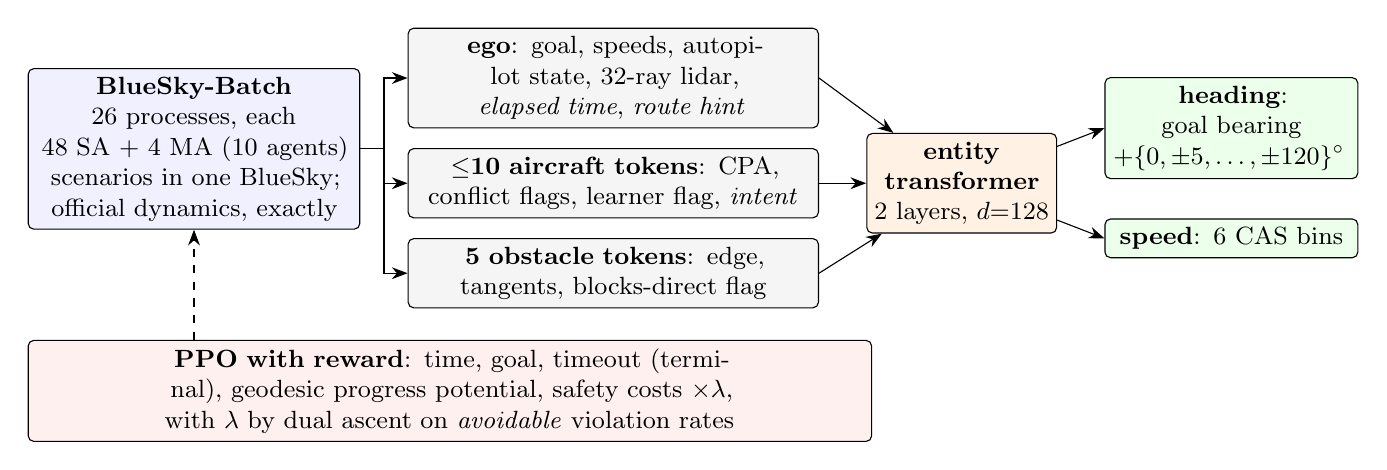
\begin{tikzpicture}[font=\small, node distance=2.5mm and 6mm,
  box/.style={draw, rounded corners=2pt, align=center, inner sep=3pt, fill=#1},
  box/.default=white, >={Stealth[length=2mm]}]
\node[box=blue!6, text width=40mm] (sim) {\textbf{\BSB}\\26 processes, each\\48 SA + 4 MA (10 agents)\\scenarios in one BlueSky;\\official dynamics, exactly};
\node[box=gray!8, right=of sim, yshift=9mm, text width=50mm] (ego) {\textbf{ego}: goal, speeds, autopilot state, 32-ray lidar, \emph{elapsed time}, \emph{route hint}};
\node[box=gray!8, below=of ego, text width=50mm] (ac) {\textbf{$\le$10 aircraft tokens}: CPA, conflict flags, learner flag, \emph{intent}};
\node[box=gray!8, below=of ac, text width=50mm] (ob) {\textbf{5 obstacle tokens}: edge, tangents, blocks-direct flag};
\node[box=orange!10, right=of ac, text width=22mm] (tf) {\textbf{entity}\\\textbf{transformer}\\2 layers, $d{=}128$};
\node[box=green!8, right=of tf, yshift=7mm, text width=30mm] (hd) {\textbf{heading}: goal bearing $+\{0,\pm5,\dots,\pm120\}^\circ$};
\node[box=green!8, right=of tf, yshift=-7mm, text width=30mm] (sp) {\textbf{speed}: 6 CAS bins};
\draw[->] (sim.east) -- ++(3mm,0) |- (ego.west);
\draw[->] (sim.east) -- ++(3mm,0) |- (ac.west);
\draw[->] (sim.east) -- ++(3mm,0) |- (ob.west);
\draw[->] (ego.east) -- (tf); \draw[->] (ac.east) -- (tf); \draw[->] (ob.east) -- (tf);
\draw[->] (tf) -- (hd.west); \draw[->] (tf) -- (sp.west);
\node[box=red!6, anchor=north west, text width=105mm] (rw) at ($(sim.west |- ob.south)+(0,-4mm)$) {\textbf{PPO with reward}: time, goal, timeout (terminal), geodesic progress potential,
 safety costs $\times\lambda$, with $\lambda$ by dual ascent on \emph{avoidable} violation rates};
\draw[->, dashed] (rw.north -| sim.south) -- (sim.south);
\end{tikzpicture}
\caption{Overview. One shared policy acts for every seat of the single-agent
(SA) and multi-agent (MA) scenarios.}
\label{fig:overview}
\end{figure*}

\section{MDP design}
\paragraph{Observation (409-D, body frame).} \emph{Ego}: goal distance and
bearing, TAS/CAS, the autopilot's selected heading and speed, sector and
obstacle status, predicted-conflict counts, a 32-ray two-channel lidar on the
true obstacle and sector polygons, the \emph{elapsed time}, and an
\emph{obstacle-aware route hint}: geodesic distance to the goal and the
steepest-descent direction of a cost-to-go field (16-connected Dijkstra on a
$96\times96$ grid per scenario, SciPy). \emph{Aircraft tokens} ($\le$10),
ranked by miss distance predicted over 300\,s: relative position and velocity,
tcpa/dcpa, predicted conflict at 120\,s and 300\,s, intrusion and learner flags,
and \emph{intent}: the active waypoint of scripted intruders (routes bend
mid-way) or the goal of other agents. \emph{Obstacle tokens} (5): nearest
boundary point, signed distance, centroid, radius, tangent bearings and
whether the obstacle blocks the direct line to the goal.

\paragraph{Action.} Two categorical choices every 10\,s: a target heading of
the bearing to the goal plus $0$, $\pm5$, $\pm12$, $\pm22$, $\pm35$, $\pm50$,
$\pm70$, $\pm90$ or $\pm120^\circ$, and a CAS of
110, 125, 140, 150, 157 or 163\,m/s (163\,m/s is the
OpenAP~\citep{sun2020openap} A320 VMO at the competition altitude). A
categorical head represents bimodal avoidance that a Gaussian would average
into a path through the conflict.

\paragraph{Reward} (0.01 = one second of flight time): $-0.01$/s; $+1$ at goal
capture; $-20$ at \emph{timeout}, terminal and not bootstrapped (with the
elapsed time observed, running out of budget is a task failure, not an
artificial truncation~\citep{pardo2018time}); a potential-based
progress term~\citep{ng1999policy} on the \emph{geodesic} route length around
RAs (the straight-line potential pulled aircraft into concave obstacle pockets,
where they timed out); per-event (2) and per-second (0.02) costs for intrusions,
RA and sector exits, each scaled by an adaptive multiplier $\lambda$; and small
soft buffers (8\,NM around aircraft, 3\,NM from obstacles and the sector edge)
and a cost per conflict predicted within 120\,s. None of these affect the
scored metrics.

\section{Learning}
\paragraph{Policy and algorithm.} Type-specific token MLPs and type embeddings
feed a 2-layer pre-LN transformer~\citep{vaswani2017attention} ($d{=}128$, 4 heads, padding masks); the
features are the ego token and a masked mean pool. Actor and critic are
separate; encoders run in bf16. PPO~\citep{schulman2017ppo} in
Stable-Baselines3~\citep{raffin2021sb3}: 292{,}864-sample rollouts, 4 epochs of
4096-sample minibatches, $\gamma{=}0.99$ per decision, GAE $0.95$, linear
learning-rate decay and annealed entropy.

\paragraph{Constrained RL on avoidable violations.} The multipliers
$\lambda_\text{intr},\lambda_\text{RA},\lambda_\text{sec}\in[1,8]$ follow dual
ascent in log space~\citep{altman1999cmdp,stooke2020pid} towards 0.02/0.01/0.005
events per episode. The generator does not keep scripted intruders 5\,NM from
the single-agent start, so some intrusions exist at $t{=}0$ and no policy can
avoid them (\S\ref{sec:failures}); counting them drives $\lambda$ to its cap
whatever the behaviour. The constraint statistic therefore \emph{excludes
violations present at spawn} (they still count in the reported metrics).

\paragraph{One policy, both tracks.} SA and MA seats are mixed in every batch,
distinguished by a mode flag and per-token learner flags; parameter sharing in
MA scenarios is self-play~\citep{yu2022mappo,dewitt2020ippo}. A finished MA seat
respawns with the official placement routine ($\ge$10\,NM from live aircraft), so
no samples are spent on dead agents, and scenarios are regenerated once the
original cohort is done, so the dense simultaneous start is trained on too. SA
scenarios use 10/12/14 intruders ($p{=}0.6/0.2/0.2$).

\paragraph{Schedule and selection.} $10^9$ steps from scratch (404-D
observation), then fine-tuning stages resumed from each other: \emph{time-aware}
(elapsed time, timeout as failure, avoidable-only constraint; best checkpoint at
1070M) and \emph{geodesic} (route potential and hint; 1070M$\to$1185M). New
input columns get zero weights, so a converted policy acts identically until
trained. Checkpoints are selected every 10M steps on 200 SA and 20 MA held-out
scenarios (seed 2024, not the reporting seed).

\begin{figure*}[t]
\centering
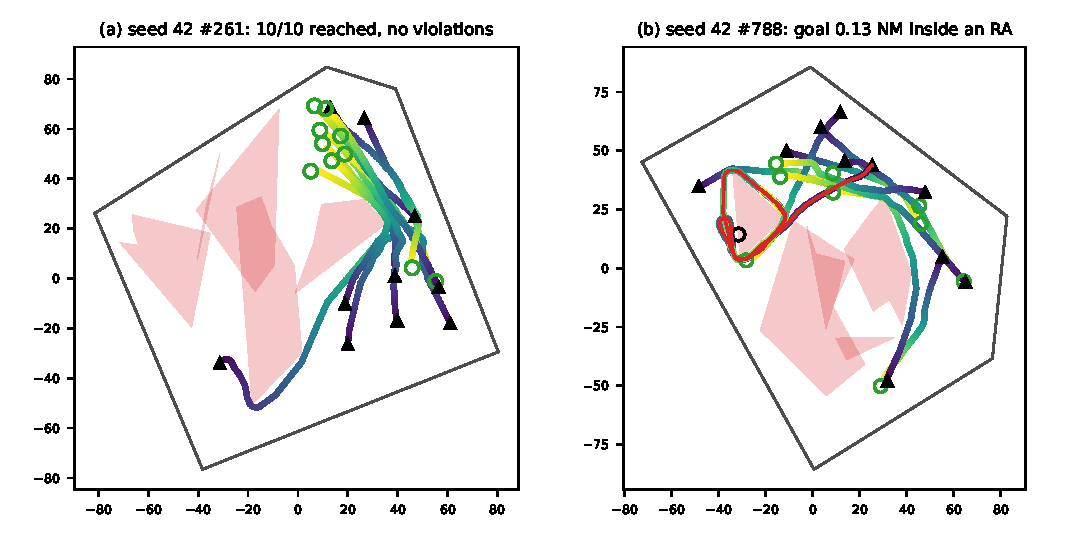
\includegraphics[width=0.78\textwidth]{figures/trajectories.pdf}
\caption{Multi-agent trajectories on seed 42 (dots coloured by time, dark =
early; grey: other traffic; shaded: restricted areas; circles: goals with the
5\,km capture radius; red: timeout). (a)~Ten aircraft with closely spaced
goals sequence in without a violation. (b)~One goal lies 0.13\,NM inside a
restricted area; the aircraft loops at its edge until the budget runs out.
\TODO{final checkpoint}}
\label{fig:traj}
\end{figure*}

\section{Results}
\begin{table}[t]
\centering\small
\caption{Official harness, seed 42, first 1000 episodes (MA: per agent-episode,
10{,}000 agent-episodes). Fly-direct is the stock environment with the zero
action. \TODO{final checkpoint}}
\label{tab:results}
\setlength{\tabcolsep}{4pt}
\begin{tabular}{@{}lrrrr@{}}
\toprule
& \multicolumn{2}{c}{Single-agent} & \multicolumn{2}{c}{Multi-agent}\\
\cmidrule(lr){2-3}\cmidrule(l){4-5}
Metric & fly-direct & ours & fly-direct & ours\\
\midrule
Goal completion [\%] & 100.0 & 99.6 & 100.0 & 99.37\\
Flight time [s] & 852.0 & 987.6 & 847.7 & 921.4\\
Intrusion events & 1.127 & 0.127 & 0.877 & 0.010\\
Intrusion time [s] & 96.3 & 5.14 & 64.8 & 0.36\\
RA events & 0.813 & 0.013 & 0.799 & 0.008\\
RA time [s] & 129.9 & 0.74 & 121.7 & 0.51\\
Sector-exit events & 0.000 & 0.008 & 0.000 & 0.005\\
Time outside sector [s] & 0.0 & 0.64 & 0.0 & 0.21\\
\bottomrule
\end{tabular}
\end{table}

Table~\ref{tab:results} gives the official results. To attribute them, every
checkpoint flies the same 1000+1000 seed-42 scenarios; MA failure changes are
paired per scenario with a scenario-cluster BCa bootstrap and SA failure changes
with an exact McNemar test (SciPy). A control continues the main run for 300M
steps without any change (Table~\ref{tab:stages}). Only the geodesic stage
reduces MA failures significantly, and its effect grew monotonically during the
fine-tune (82$\to$72$\to$63$\to$62 failures at 1087M, 1165M, 1177M, 1185M)
while safety events stayed at 0.022--0.025 per aircraft. SA failures
(8$\to$4) are not significantly different ($p{=}0.29$). Against the
time-aware control, which trained twice as long (230M vs 115M steps), the
geodesic checkpoint has 17 fewer MA failures per 1000 scenarios [5, 31]; the
control reaches 3 SA failures, so on an equal SA/MA weighting of
$100\,g - 10\,v - 0.01\,t$ (goal, violations, flight time) the two tie
($+0.02$ [$-0.22$, $+0.21$]).

\begin{table}[t]
\centering\small
\caption{Stage contributions on seed 42 (same scenarios for every row).
$\Delta$: change in MA failures per 1000 scenarios versus the main checkpoint,
95\% CI.}
\label{tab:stages}
\setlength{\tabcolsep}{3pt}
\begin{tabular}{@{}lrrl@{}}
\toprule
Checkpoint & SA fail. & MA fail. & $\Delta$ MA [95\% CI]\\
& /1000 & /10{,}000 & \\
\midrule
main (950M, selected) & 8 & 83 & ---\\
\quad +300M steps, no change & 9 & 88 & $+5$ [$-8$, $+19$]\\
\quad +avoidable-only constraint & 5 & 75 & $-8$ [$-21$, $+4$]\\
time-aware (1070M) & 9 & 78 & $-5$ [$-22$, $+11$]\\
\quad +230M steps, no change & 3 & 79 & $-4$ [$-21$, $+12$]\\
\textbf{geodesic (1185M)} & \textbf{4} & \textbf{62} & $\mathbf{-21}$ [$-41$, $-5$]\\
\bottomrule
\end{tabular}
\end{table}

\section{Failure analysis}\label{sec:failures}
\paragraph{SA violations are mostly unavoidable.} We replayed every violating
episode exactly and branched each of the 102 actions 10--160\,s before the
onset (a diagnostic; the controller stays the RL policy). Of 151 intrusions on
1000 fresh episodes, 116 exist at $t{=}0$ (the intruder spawns within 5\,NM); an
escape was found for 18 of the other 35, and for 12/15 RA and 7/8 sector-exit
events. \TODO{numbers from a 490M checkpoint; re-run on the final one}

\paragraph{Every failure is a timeout; half of the MA ones are goals inside
RAs.} All failures exhaust the 3000\,s budget. Of 10{,}000 MA goals on seed~42,
29 lie \emph{inside} an RA and none is reached: 23 deeper than the 5\,km capture
radius (reachable only by entering) and 6 shallower (capturable from outside).
Table~\ref{tab:failures} classifies failures on seed~42 and on 70k fresh
(agent-)episodes. We decided \emph{not} to enter RAs for the deep goals, which
would gain $\sim$0.3 points of MA completion at the cost of safety events.
For shallow goals the policy does poorly (Fig.~\ref{fig:traj}b): on 249 held-out scenarios it reaches
14\% of them and enters the area in 37\% of cases ($\sim$50$\times$ its usual
rate), because its route hint aims at the goal point inside the area while the
safety cost keeps it out. \emph{Fix:} the route field targets the nearest
point just outside the area when the goal is less than 5\,km inside, and we
fine-tune with prioritized replay~\citep{jiang2021plr} of mined hard scenarios
(shallow-goal MA scenarios, MA timeouts, SA timeouts and the slowest 5\%;
scenarios with deep goals are excluded, so replay never rewards an entry).
\TODO{results}

\begin{table}[t]
\centering\small
\caption{Failure classes (all timeouts): seed 42 and fresh mined episodes.}
\label{tab:failures}
\setlength{\tabcolsep}{3pt}
\begin{tabular}{@{}lrrrr@{}}
\toprule
& \multicolumn{2}{c}{MA} & \multicolumn{2}{c}{SA}\\
\cmidrule(lr){2-3}\cmidrule(l){4-5}
Goal location & seed 42 & 50k & seed 42 & 20k\\
\midrule
inside RA, deeper than 5\,km & 23 & 94 & 1 & 16\\
inside RA, capturable outside & 6 & 34 & 0 & 6\\
within 10\,NM of an RA & 1 & 9 & 1 & 0\\
far from RAs (congestion loops) & 32 & 196 & 2 & 64\\
\bottomrule
\end{tabular}
\end{table}

\paragraph{Remaining inefficiency is a tail.} Against each flight's geodesic
route length at the policy's own 90th-percentile clear-path speed, the excess
is 139\,s (SA) and 81\,s (MA) per flight, half of it from the slowest 10\%
(loops near the start, waiting for traffic, long detours). These flights
reverse turn side twice as often, but decoding with hysteresis does not help:
only a weak bonus is neutral-to-positive ($+0.13$ selection score on seed~42,
CI [0.00, 0.38], chosen on another seed) and strong commitment lengthens
flights, so reversals are mostly purposeful steering. Biasing decoding towards
top speed and the direct heading raises MA violations by 45\% without fewer
failures: the learned trade-off is not over-cautious. Uniform weight averaging
of the last three checkpoints~\citep{wortsman2022soups} changes nothing.

\section{Limitations}
One training seed per configuration: paired tests control for scenario noise,
not seed variance \TODO{seed repeats}. The generator occasionally places goals
inside RAs; we report them rather than trade safety for completion. The
selection score is our own; the judges weigh the metrics jointly.

\paragraph{Reproducibility.} Code, trained model and per-episode CSVs:
\TODO{repository link}. Table~\ref{tab:results} is reproduced by
\texttt{python -m scripts.evaluate\_competition -{}-env sa|ma -{}-model
<model>}.

{\small
\bibliographystyle{unsrtnat}
\bibliography{refs}}
\end{document}
